\documentclass[11pt]{article}
\usepackage[margin=1in]{geometry}
\usepackage{graphicx,amsmath,amssymb}
\usepackage[numbers,super,sort&compress]{natbib}
\usepackage{xcolor}
\usepackage{authblk}
\usepackage{caption}
\usepackage{siunitx}
\usepackage[colorlinks=true,allcolors=blue]{hyperref}
\captionsetup{font=small,labelfont=bf}

% ---- placeholder macro for fill-later content ----
\newcommand{\TODO}[1]{{\color{red}\textbf{[TODO: #1]}}}
\newcommand{\PLACEHOLDER}[1]{{\color{orange}\textbf{[PLACEHOLDER --- #1]}}}
\graphicspath{{../figures/}}

\title{\textbf{TFScope: sequence-only prediction of transcription-factor\\ binding specificity rivals structure-based methods}}
\author[1]{Lei Huang}
\author[1]{\TODO{co-authors}}
\author[1,*]{\TODO{corresponding author}}
\affil[1]{\TODO{affiliations}}
\affil[*]{Correspondence: \TODO{email}}
\date{}

\begin{document}
\maketitle

% =====================================================================
\begin{abstract}
\noindent
Predicting the DNA sequence preference of a transcription factor (TF) from its
protein sequence alone remains a central problem in gene-regulatory genomics.
State-of-the-art accuracy is achieved by structure-based models that require an
experimentally determined or predicted protein--DNA complex, limiting their use
for the large fraction of TFs and designed proteins that lack a reliable
structure. Here we introduce \textbf{TFScope}, a sequence-only model that maps a
TF DNA-binding domain (DBD) to a position weight matrix (PWM) using a
\emph{frozen} protein language model (ESM-2 650M) adapted with low-rank
(LoRA) fine-tuning, a residue mixture-of-experts, and a contact-aware motif head.
On a leakage-controlled benchmark in which held-out TFs share no training
identity, a five-seed TFScope ensemble reaches a motif content correlation of
$0.664$ and is statistically indistinguishable from the structure-based method
DeepPBS (mean gate-oracle $r$ $0.657$ vs $0.626$; bootstrap $p=0.30$), despite
using no structure at inference. An independent structure predictor (Boltz-2)
judges TFScope's sequence-only consensus motifs to form protein--DNA complexes at
least as confidently as DeepPBS's ($\text{ipTM}\ 0.957$ vs $0.923$; $32/41$ TFs;
Wilcoxon $p=1\times10^{-5}$). Probing the frozen backbone shows that it linearly
encodes DNA-contact residues (AUROC $0.95$) and organizes DBD families
(k-NN purity $0.83$), explaining where the signal comes from; a variance
decomposition attributes $59\%$ of TFScope's edge to genuine within-family
specificity rather than family lookup. We further show directional
single-mutation motif switching (MyoD1 E-box) and application to \emph{de novo}
designed DBDs, and we transparently characterize the model's principal
limitation --- insensitivity to specificity-altering point mutations inherited
from the frozen backbone. TFScope makes accurate specificity prediction available
wherever only a protein sequence is known.
\end{abstract}

\vspace{1em}

% =====================================================================
\section*{Introduction}

Transcription factors (TFs) interpret the genome by binding short, degenerate DNA
motifs, and the position weight matrix (PWM) that summarizes this preference is
one of the most widely used objects in regulatory genomics. PWMs drive motif
enrichment analysis, the annotation of \emph{cis}-regulatory elements, and the
interpretation of non-coding variants, and they anchor the priors used by many
chromatin and gene-expression models\cite{weirauch2014cisbp,castromondragon2022jaspar,avsec2021enformer}.
A PWM is therefore not merely a descriptive statistic but a reusable input to a
large downstream ecosystem, which makes the availability of accurate PWMs a
practical bottleneck rather than an academic curiosity.

Yet measured specificities remain sparse. High-throughput assays such as
protein-binding microarrays and HT-SELEX have characterized many TFs, but the
experiments are laborious and have covered only a fraction of the roughly 1,600
human TFs, with even thinner coverage across non-model organisms\cite{jolma2013dna,weirauch2014cisbp}.
The gap is widening rather than closing, because protein design now produces
\emph{de novo} DNA-binding proteins far faster than any binding assay can profile
them. A model that predicts a PWM directly from a protein sequence would let this
downstream ecosystem operate wherever a sequence is known, including the majority
of TFs and essentially all designed proteins that will never be assayed.

Computational specificity prediction has followed two routes with complementary
weaknesses. Structure-based models read the physicochemical readout of a
protein--DNA complex and currently define the state of the art; the geometric
deep-learning method DeepPBS, for example, predicts specificity from the geometry
and chemistry of the interface\cite{mitra2024deeppbs}. Their accuracy, however, is
gated on the availability and quality of a structure. For a TF without a
co-crystal, and for any designed protein, a complex must first be predicted, which
adds computational cost and a second, compounding source of error. Sequence-only
models avoid this dependency but have historically been less accurate, and their
reported advantages are frequently inflated by TF leakage, in which test proteins
share close homologs with the training set and the model succeeds by recall rather
than by genuine generalization\cite{mitra2024deeppbs}. Distinguishing real
sequence-to-specificity inference from leakage is thus as important as raw
accuracy.

Protein language models (PLMs) trained on evolutionary-scale sequence data have
reshaped what is achievable from sequence alone, recovering contacts, structure,
and function that were previously thought to require experimental
input\cite{rives2021esm1b,lin2023esm2}. We reasoned that a frozen PLM might already
encode the recognition information that specifies DNA binding, and that the
remaining problem is not representation learning but read-out: extracting a
calibrated motif from features the backbone has already computed. This framing
predicts that a small, structure-free adapter on a frozen backbone should suffice,
and that the ceiling on accuracy should be set by the backbone rather than by the
adapter.

Here we test this hypothesis with \textbf{TFScope}, a sequence-only model that maps
a TF DNA-binding domain to a PWM through a frozen ESM-2 650M backbone and a
lightweight contact-aware adapter. Under strict leakage control, TFScope reaches
accuracy parity with the structure-based method DeepPBS without ever seeing a
structure at inference. An independent structure predictor, blind to both models,
judges TFScope's sequence-only motifs to form protein--DNA complexes at least as
confident as those from DeepPBS. Probing the frozen backbone shows why this is
possible and where the signal originates, a variance decomposition establishes that
the model reads specificity within TF families rather than merely retrieving a
family average, and we characterize transparently the one regime, single
specificity-altering point mutations, where a frozen backbone remains limited.

% =====================================================================
\section*{Results}

\subsection*{A structure-free model of transcription-factor specificity}

TFScope maps a TF DNA-binding domain (DBD) to a $4\times L$ PWM in a single forward
pass, using no structural input at any stage of inference (Fig.~\ref{fig:overview}).
The design follows directly from the read-out hypothesis: because we assume the
recognition information already exists in the backbone, we keep the backbone frozen
and invest the model's limited capacity in extracting and calibrating a motif from
it. Concretely, per-residue features are taken from a frozen ESM-2 650M
encoder\cite{lin2023esm2} as a learned weighted average of its last four
transformer layers, which lets the model draw on both the syntactic features of
late layers and the more local features of earlier ones, and each residue is tagged
with a binary indicator of whether it lies inside the annotated DBD.

Four lightweight components then convert these frozen features into a PWM. Low-rank
adaptation\cite{hu2022lora} (LoRA, rank 16) supplies the only updates that touch the
backbone, adapting attention projections at a small parameter cost while leaving the
pretrained representation intact. A token-level residue mixture-of-experts, with two
shared and eight routed experts conditioned on a TF family embedding, allows
different structural classes of DBD to be processed by specialized parameters
without fragmenting the model into per-family heads. Dual gated-attention pooling
then summarizes the residues twice, once globally and once restricted to the DBD, so
that the motif read-out sees both the domain context and the recognition surface.
Finally, a position gate head emits a soft gate over motif positions together with a
pooled protein representation, and a contact-aware PWM head predicts a prior PWM and
adds a learned correction, so that the final motif is the sum of a coarse prior and a
contact-informed refinement. The correction is the only place structural knowledge
enters the model, and it does so only during training, through supervision from
recognition-residue DNA contacts; at inference the head runs from sequence alone.

TFScope is trained on curated protein-to-PWM pairs using DBD-cropped inputs, so that
the model learns to read the recognition domain rather than incidental flanking
sequence. Because single models are sensitive to the arbitrary register in which a
short motif is committed, we report a five-seed ensemble whose members are aligned to
a common reference frame by offset and reverse-complement before averaging, which
removes register disagreement and yields a more stable motif than any single seed.
Full architecture, training, and ensembling details are given in Methods.

\subsection*{TFScope enables specificity prediction without structure}

To ask whether sequence-only prediction can rival a structure-based model, we
benchmarked TFScope against DeepPBS\cite{mitra2024deeppbs} on a shared held-out set
(Fig.~\ref{fig:benchmark}). The comparison is only meaningful if leakage is
controlled, because naive splits reward a model for recognizing a training homolog
rather than for generalizing to a new protein. We therefore imposed two independent
controls. First, we used a held-out set clustered at 40\% DBD identity, so that test
proteins are not close homologs of any training protein. Second, for the direct
head-to-head we retrained DeepPBS after removing the benchmark genes from its
training data, producing a gene-disjoint comparison in which neither model has seen
the test TFs. Throughout, we scored PWMs with a register-invariant, oracle-aligned
motif-content correlation that permits an offset and reverse-complement before
comparison, the appropriate metric for methods that do not share DeepPBS's fixed
crystallographic coordinate frame; scoring in a fixed frame would penalize a
sequence-only method for register alone rather than for the motif it predicts.

On the clustered holdout (84 structures spanning 41 TFs), the five-seed TFScope
ensemble reached a motif-content correlation of $\mathbf{0.664}$, ahead of the
single-seed model ($0.629$) and of every intermediate configuration in an ablation
ladder that adds the model's components one at a time (Fig.~\ref{fig:benchmark}).
Against DeepPBS under the matched per-motif protocol, TFScope scored $0.657$ and
DeepPBS $0.626$, a paired difference of $+0.031$ that a bootstrap test does not
distinguish from zero ($p=0.30$). The two methods are therefore statistically
indistinguishable, with the point estimate favoring the sequence-only model. The
gene-disjoint retrain gave the same conclusion from the opposite direction: the
retrained DeepPBS ensemble scored $0.720$ and TFScope $0.685$ on those 20 genes, a
gap of $0.034$ whose confidence interval crosses zero. We note that the frequently
quoted pretrained-DeepPBS value of $0.806$ is not a valid comparison here, because
those checkpoints were trained on all 20 test genes and the number reflects leakage
rather than generalization. Taken together, and consistent across two orthogonal
leakage controls, TFScope attains structure-level accuracy while using no structure
at inference. Per-family performance (Fig.~\ref{fig:perfamily}) shows that parity is
broad rather than driven by a single easy family, spanning homeodomain, bHLH, bZIP,
ETS, C2H2 zinc-finger, and nuclear-receptor DBDs, and representative predicted logos
recover the canonical motifs of held-out TFs (Fig.~\ref{fig:logos}).

\subsection*{Predicted motifs form confident protein--DNA complexes}

A correlation-based benchmark measures agreement with a reference PWM, but it cannot
say whether a predicted motif is biophysically sensible, and it inherits any bias in
the reference. We therefore sought an orthogonal, model-independent assay of motif
quality by asking a question that neither TFScope nor DeepPBS was optimized to
answer: does the DNA a model predicts actually form a confident complex with its own
TF? For each of the 41 benchmark TFs we folded the protein together with its
TFScope-ensemble consensus DNA and, separately, together with its DeepPBS consensus
DNA, using Boltz-2\cite{wohlwend2024boltz} with ColabFold multiple-sequence
alignments\cite{mirdita2022colabfold}. Because the protein is identical within each
pair, the comparison isolates the effect of the predicted DNA on the confidence of
the modeled interface (ipTM).

TFScope's sequence-only motifs formed complexes at least as confident as DeepPBS's
structure-derived motifs, and by a margin that is small per TF but highly consistent
across the set (mean ipTM $\mathbf{0.957}$ versus $0.923$; mean difference $+0.035$;
TFScope favored in $\mathbf{32}$ of $41$ TFs; Wilcoxon $p=1\times10^{-5}$; mean
complex pLDDT $0.948$ versus $0.921$; Fig.~\ref{fig:foldability}). The effect is not
an artifact of motif length, since the per-TF difference in ipTM is if anything
weakly anti-correlated with the difference in DNA length (Spearman $\rho=-0.43$).
Boltz-2 has no knowledge of either predictor and was not involved in training or
scoring, so this result is independent evidence that TFScope's sequence-only read-out
is not merely correlated with reference PWMs but is physically coherent, producing DNA
that its cognate TF can bind in a confidently modeled complex.

\subsection*{A frozen language model encodes DNA-recognition signals}

The parity results raise a mechanistic question: if the backbone is frozen and the
adapter is small, where does the recognition signal come from? The read-out
hypothesis makes a testable prediction, namely that the information TFScope needs
should be linearly decodable from the frozen backbone before any specificity
training. We tested this directly by probing frozen ESM-2 embeddings for two kinds
of knowledge that a specificity model would need.

First, a linear probe on frozen residue embeddings predicts which DBD residues
contact DNA, defined as residues within \SI{4.5}{\angstrom} of DNA in co-crystal
structures, with a pooled AUROC of $\mathbf{0.95}$ and AUPRC of $0.78$ across 2,324
complexes and 240,072 residues, evaluated with grouping by protein sequence so that
no TF is shared between training and test folds (Fig.~\ref{fig:recognition}). The
backbone thus already knows, from sequence alone, which residues form the recognition
interface. Rendered onto a homeodomain--DNA co-crystal (PBX1, PDB 1B72), the residues
the probe scores as DNA-contacting are precisely those of the recognition helix that
inserts into the major groove and hydrogen-bonds to the bases, matching the true
crystallographic contacts (Fig.~\ref{fig:recognition}). Second, the same frozen
embeddings organize TFs by structural family, with a k-nearest-neighbor purity of
$0.83$ and a linear family-probe accuracy of $0.96$, so that clade identity is also
available without supervision. Both signals are present before any TFScope training,
which supports the view that the backbone supplies the recognition content and the
contact-aware head mainly converts it into a calibrated, position-resolved motif.
This also explains two negative results reported below, that a more elaborate
biophysical head does not improve on the simple one and that a weaker backbone
degrades accuracy: the informative bottleneck is the frozen representation, not the
read-out.

\subsection*{TFScope resolves specificity within transcription-factor families}

Because the backbone encodes family identity so cleanly, a natural worry is that
TFScope succeeds trivially, by recognizing a TF's family and returning that family's
average motif. Many members of a family do share a core motif, so a family-lookup
model would still score well on aggregate benchmarks while learning nothing about the
individual protein. We tested this directly by decomposing TFScope's advantage over a
random real-PWM baseline into the part explained by family identity and the part that
requires resolving differences between members of the same family. On the clustered
holdout, family identity accounts for $41\%$ of the advantage, but the majority,
$\mathbf{59\%}$, reflects genuine within-family specificity (permutation
$p=2\times10^{-4}$; Fig.~\ref{fig:mutagenesis}). TFScope therefore reads binding
preference at the level of the individual protein, distinguishing paralogs that a
family-average model would collapse, rather than performing family lookup.

\subsection*{TFScope captures mutational rewiring and designed proteins}

Two applications probe whether TFScope generalizes beyond reproducing the motifs of
natural TFs. The first is mutational rewiring, in which a single amino-acid change
alters specificity. Using a directional switch score that measures the shift in
preference between two candidate sites rather than the raw motif magnitude, TFScope
reproduces the E-box switch that the L122R substitution induces in MyoD1
($\Delta_{\mathrm{switch}} = +9.17$; Fig.~\ref{fig:switch}), and an independent
structure-based ensemble median agrees that the mutant prefers the canonical
\texttt{CACGTG} site. This shows that the model can register the qualitative
consequence of a substitution even though, as we quantify below, it does not
reliably capture the fine magnitude of every point mutation.

The second application is prediction for proteins that do not exist in nature.
Applied to a panel of \emph{de novo} designed DBDs, TFScope recovers the intended
CAC-type preference to a graded degree, most clearly for the design DBP6, where the
predicted motif correlates with the intended target at $r=0.65$ (Fig.~\ref{fig:dbp}).
Because designed proteins have no homologs in the training data and no measured
specificities, this is a stringent test of generalization and a setting where a
structure-based pipeline would additionally require a predicted complex. TFScope
provides a first-pass specificity readout for such designs directly from sequence.
\PLACEHOLDER{expand designed-DBP paragraph with the remaining design cases and any
experimental validation once finalized}

\subsection*{Point-mutation sensitivity is bounded by the frozen backbone}

The same design choice that makes TFScope general also bounds it in one regime, and
we characterize this limit transparently rather than leaving it for readers to
discover. On the Barrera panel of homeodomain wild-type and mutant
pairs\cite{barrera2016survey}, in which single substitutions produce measurable
changes in specificity, TFScope is largely insensitive to the mutation: it predicts a
mean absolute change in the motif of $0.005$ against an observed change of $0.180$,
and its predicted changes are essentially uncorrelated with the measured ones. The
cause is structural. A single substitution moves the frozen ESM-2 representation only
slightly, so a read-out built on that representation under-responds to individual
residue changes, even though it captures family- and clade-level preferences well.
This limit is consistent with the successful switch score of the previous section,
because that score reads a coarse, directional preference between two sites, whereas
the Barrera comparison demands the fine magnitude of each perturbation. Closing this
gap without giving up the model's structure-free generality, for example by
introducing backbone features that respond to individual residues, is the central
open problem we discuss next.

% =====================================================================
\section*{Discussion}

TFScope shows that accurate prediction of TF binding specificity does not require a
protein--DNA structure. A frozen protein language model already carries the
recognition signal, and a small structure-free adapter is enough to read it out to
motif-level accuracy that matches a strong structure-based method under strict
leakage control. This result matters less as a leaderboard update than as a change in
what is required to obtain a PWM: the large downstream ecosystem that consumes PWMs
can now be driven from sequence alone, wherever a DBD sequence is known.

Two features make the parity credible rather than a metric artifact. We controlled TF
leakage explicitly, using both a homology-clustered holdout and a gene-disjoint
retrain of the competing method, and observed parity under both; leakage is the most
common reason that sequence-only comparisons have been unreliable, and removing it did
not erase the result. We also validated the predictions with an assay that is
independent of both models, folding each predicted motif with its TF and finding that
TFScope's sequence-only DNA forms complexes at least as confident as the
structure-derived DNA. Agreement between a reference-based benchmark and a
reference-free biophysical assay is stronger evidence than either alone.

The interpretability analyses locate the signal and reframe what the model is doing.
The frozen backbone linearly encodes both DNA-contact residues and family identity,
and TFScope's advantage over baselines is majority within-family rather than family
lookup, so the model reads specificity at the level of the individual protein while
drawing on representations that were never trained for DNA binding. A practical
implication is that the backbone, not the adapter, sets the ceiling. Two negative
results support this reading: replacing the simple motif head with a more elaborate
biophysical recognition-energy decoder did not improve accuracy, and substituting a
weaker backbone reduced it. Effort is therefore better spent on the representation
than on the read-out.

The same analysis explains the model's principal limitation. Because a single
substitution barely moves a frozen ESM-2 representation, TFScope under-reads the fine
magnitude of specificity-altering point mutations, even as it captures family- and
clade-level preferences and the directional consequences of some substitutions.
Progress most likely requires backbone features that respond to individual residues,
for instance contact- or structure-conditioned representations, obtained without
reintroducing a hard structure dependency at inference; supplying such structural
information only during training, as our contact-aware correction already does, is one
promising direction. \PLACEHOLDER{position relative to concurrent PLM-based
specificity work once the literature search is complete}

For practitioners, TFScope turns specificity prediction into a single forward pass on
a protein sequence, with no structure required at inference. This is most valuable
exactly where structure-based methods are weakest, for the many TFs without a
co-crystal and for the rapidly growing space of designed DNA-binding proteins, and it
positions sequence-only prediction as a default first step whose motifs can then be
refined or validated by structure when one is available.

% =====================================================================
\section*{Methods}
\small

\subsection*{Model architecture}
Frozen ESM-2 650M (\texttt{esm2\_t33\_650M\_UR50D}) backbone; per-residue features
are a learned weighted average of the last four transformer layers, concatenated
with a binary DBD indicator. Adaptation: LoRA adapters (rank 16); a token-level
residue mixture-of-experts with 2 shared and 8 routed experts, conditioned on a
family embedding; dual gated-attention pooling (a global pool and a
DBD-restricted pool); a position gate head with a projection head emitting a soft
motif gate (up to 20 positions) and a pooled protein representation; and a
contact-aware PWM head producing a prior PWM plus a contact-aware correction
(Final PWM $=$ Prior $+$ Correction). The correction is supervised with
recognition-residue DNA-contact labels during training only; at inference the
model is sequence-only. Output is a $4\times L$ PWM with the gate.
\TODO{exact LoRA target modules, MoE routing/top-k, gated-attention and
correction equations, param counts, weighted-layer indices}

\subsection*{Training data and splits}
Protein$\rightarrow$PWM pairs from \texttt{tf\_pwm\_training\_v23} with DBD-cropped
inputs (\texttt{dbd\_start}=0). Held-out evaluation uses a 40\%-DBD-identity
clustered split and a gene-disjoint $20$-gene set for the DeepPBS comparison.
\TODO{data sources (JASPAR/HT-SELEX/CIS-BP), counts per family, dedup/clustering
procedure, exact train/val/test sizes}

\subsection*{Ensembling}
Five seeds (42/1/7/13/23). Each member commits its own motif core via the span
gate; members are register-aligned to the seed-42 core (offset $\pm10$,
reverse-complement, minimum overlap 3) and the aligned PWMs are averaged and
renormalized.

\subsection*{Evaluation metrics}
Panel A: oracle-aligned motif \emph{content} correlation (register-invariant,
$r$). Panel B: end-to-end coverage-aware correlation (covR) with the learned
gate. Mean/median gate-oracle-$r$ aligns each method's IC core to ground truth
before scoring. \TODO{precise metric definitions + equations}

\subsection*{DeepPBS comparison}
DeepPBS\cite{mitra2024deeppbs} run in a dedicated environment
(\TODO{torch/PyG versions}); \texttt{prot\_shape} inputs; 5-model ensemble.
Gene-disjoint retrain removes the $20$ benchmark genes from training. The
pretrained checkpoints are leakage-contaminated for this benchmark and reported
only as a reference.

\subsection*{Foldability assay}
For each of $41$ TFs, the protein was folded with (a) its TFScope-ensemble
consensus dsDNA and (b) its DeepPBS consensus dsDNA using
Boltz-2\cite{wohlwend2024boltz} (ColabFold MSA server\cite{mirdita2022colabfold};
identical protein per pair, so MSAs are reused). Interface confidence (ipTM) and
complex pLDDT were read from Boltz confidence outputs. Length control: Spearman
correlation of $\Delta$ipTM with $\Delta$motif-length.

\subsection*{Contact-residue and family probes}
Frozen layer-33 residue embeddings; linear probe for DNA-contact residues
(\SI{4.5}{\angstrom} cutoff from co-crystals), GroupKFold by protein sequence,
$2{,}324$ complexes. Family organization: k-NN purity and linear family probe on
frozen DBD embeddings. PyMOL renders write the contact-probe score into the
B-factor column of PDB 1B72.

\subsection*{Within-family decomposition}
\TODO{describe permutation procedure separating family-identity vs within-family
contributions to the edge over a random-real-PWM baseline}

\subsection*{Mutation sensitivity and switch score}
Barrera\cite{barrera2016survey} wild-type/mutant homeodomain pairs; mean absolute
PWM change vs measured specificity change. Directional switch score:
\TODO{definition of $\Delta_{\mathrm{switch}}$}.

\subsection*{Statistics}
Bootstrap and Wilcoxon signed-rank tests as noted; permutation test for the
variance decomposition. \TODO{n, seeds, CI method, multiple-comparison handling}

\subsection*{Code and data availability}
\TODO{repository URL, checkpoint DOI, processed-data deposition}

\normalsize
% =====================================================================
\section*{Declarations}
\noindent\textbf{Author contributions (CRediT).} \TODO{fill per author}\\
\textbf{Competing interests.} The authors declare no competing interests. \TODO{confirm}\\
\textbf{Funding.} \TODO{grants}\\
\textbf{Data availability.} \TODO{deposition + accession}\\
\textbf{Code availability.} \TODO{repo + license}\\
\textbf{AI-use statement.} \TODO{per Nature Methods policy; drafting assistance used}

% =====================================================================
\section*{Figures}

\begin{figure}[h]\centering
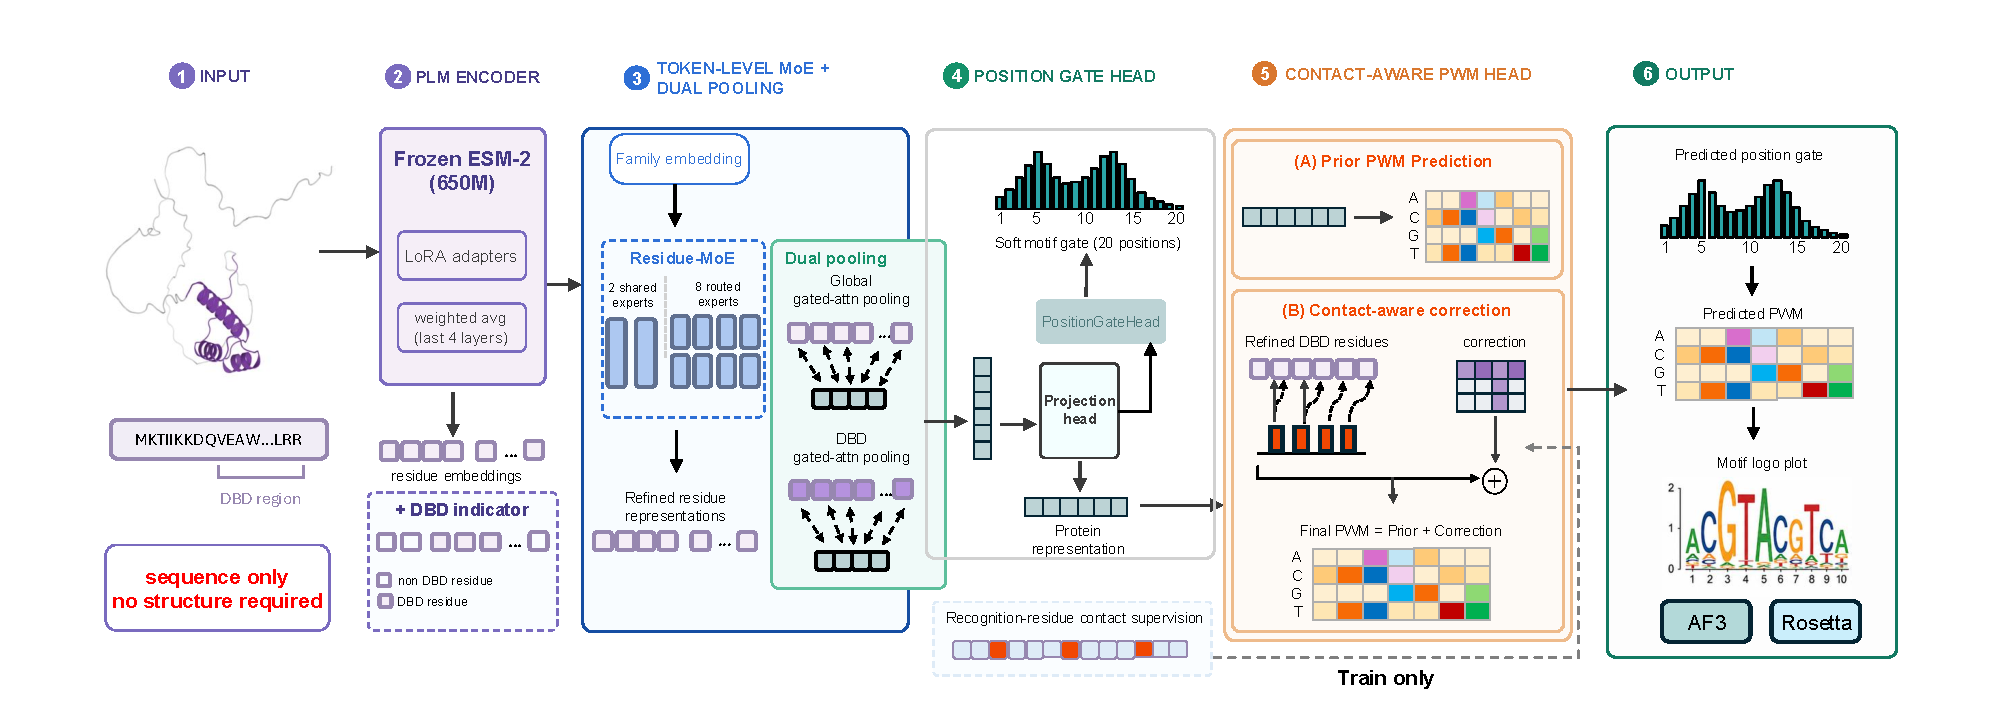
\includegraphics[width=\linewidth]{Model.pdf}
\caption{\textbf{TFScope architecture (sequence-only, no structure at inference).}
(1)~Input: a TF DNA-binding-domain (DBD) protein sequence. (2)~PLM encoder: a
\emph{frozen} ESM-2 650M backbone with LoRA adapters; residue embeddings are a
weighted average of the last four layers, concatenated with a DBD indicator.
(3)~Token-level residue mixture-of-experts (2 shared $+$ 8 routed experts)
conditioned on a family embedding, followed by dual gated-attention pooling
(global and DBD-restricted). (4)~Position gate head: a projection head produces a
soft motif gate over positions and a protein representation. (5)~Contact-aware
PWM head: a prior PWM (A) is refined by a contact-aware correction (B) driven by
recognition-residue contact supervision (train-only), giving Final PWM $=$ Prior
$+$ Correction. (6)~Output: the predicted position gate, PWM, and motif logo;
predicted consensus DNA can be validated by downstream folding (AF3/Boltz) or
Rosetta.}
\label{fig:overview}
\end{figure}

\begin{figure}[h]\centering

\includegraphics[width=0.7\linewidth]{figure1c_best_logos.png}
\caption{\textbf{Representative predicted motifs.} TFScope-ensemble predicted
logos for held-out TFs. \label{fig:logos}}
\end{figure}

\begin{figure}[h]\centering

\includegraphics[width=0.85\linewidth]{figure1e_perfamily_benchmark84.png}
\caption{\textbf{Leakage-controlled benchmark, per family.} Motif content
correlation on the clustered holdout ($n{=}84$, $41$ TFs); ensemble $0.664$.
Head-to-head with DeepPBS is a statistical tie (mean gate-oracle $r$ $0.657$ vs
$0.626$; bootstrap $p=0.30$). \label{fig:perfamily}}
\end{figure}
% NOTE: dedicated benchmark bar/ladder panel (\ref{fig:benchmark}) still to be assembled
\begin{figure}[h]\centering
\PLACEHOLDER{benchmark bar + ablation ladder panel}
\caption{\textbf{Benchmark and ablation ladder.} \TODO{assemble from
results/iclr\_phase1\_apples\_to\_apples}. \label{fig:benchmark}}
\end{figure}

\begin{figure}[h]\centering
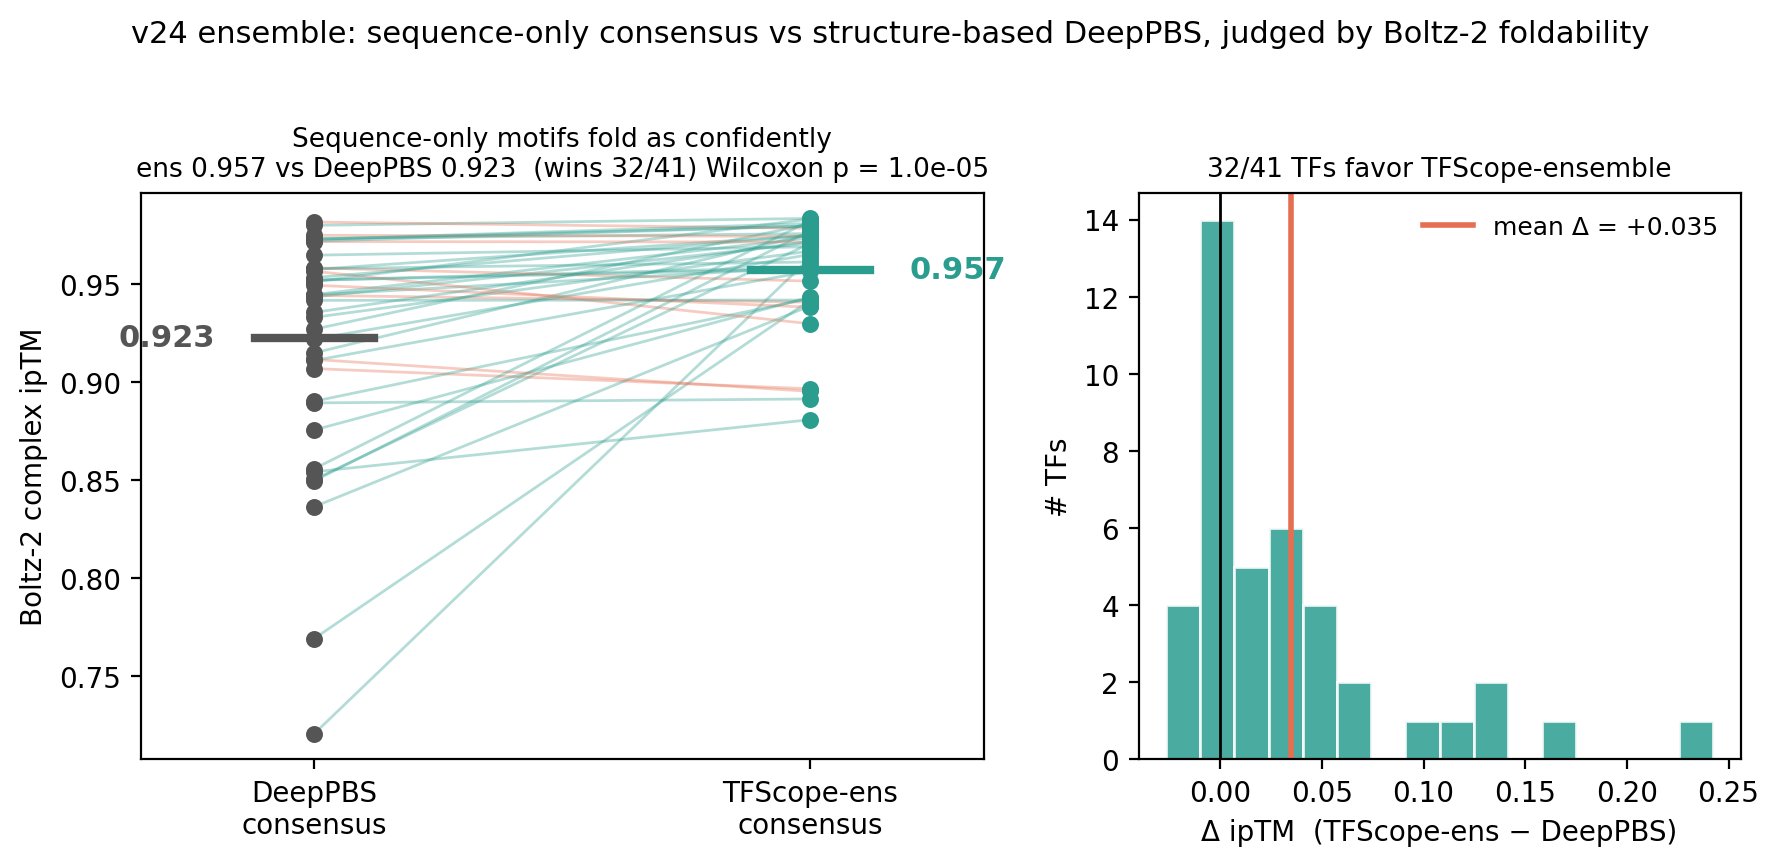
\includegraphics[width=0.9\linewidth]{figure_foldability.png}
\caption{\textbf{Independent foldability.} Boltz-2 complex ipTM for TFScope-
ensemble vs DeepPBS consensus DNA ($41$ TFs): $0.957$ vs $0.923$, $32/41$ favor
TFScope, Wilcoxon $p=1\times10^{-5}$. \label{fig:foldability}}
\end{figure}

\begin{figure}[h]\centering
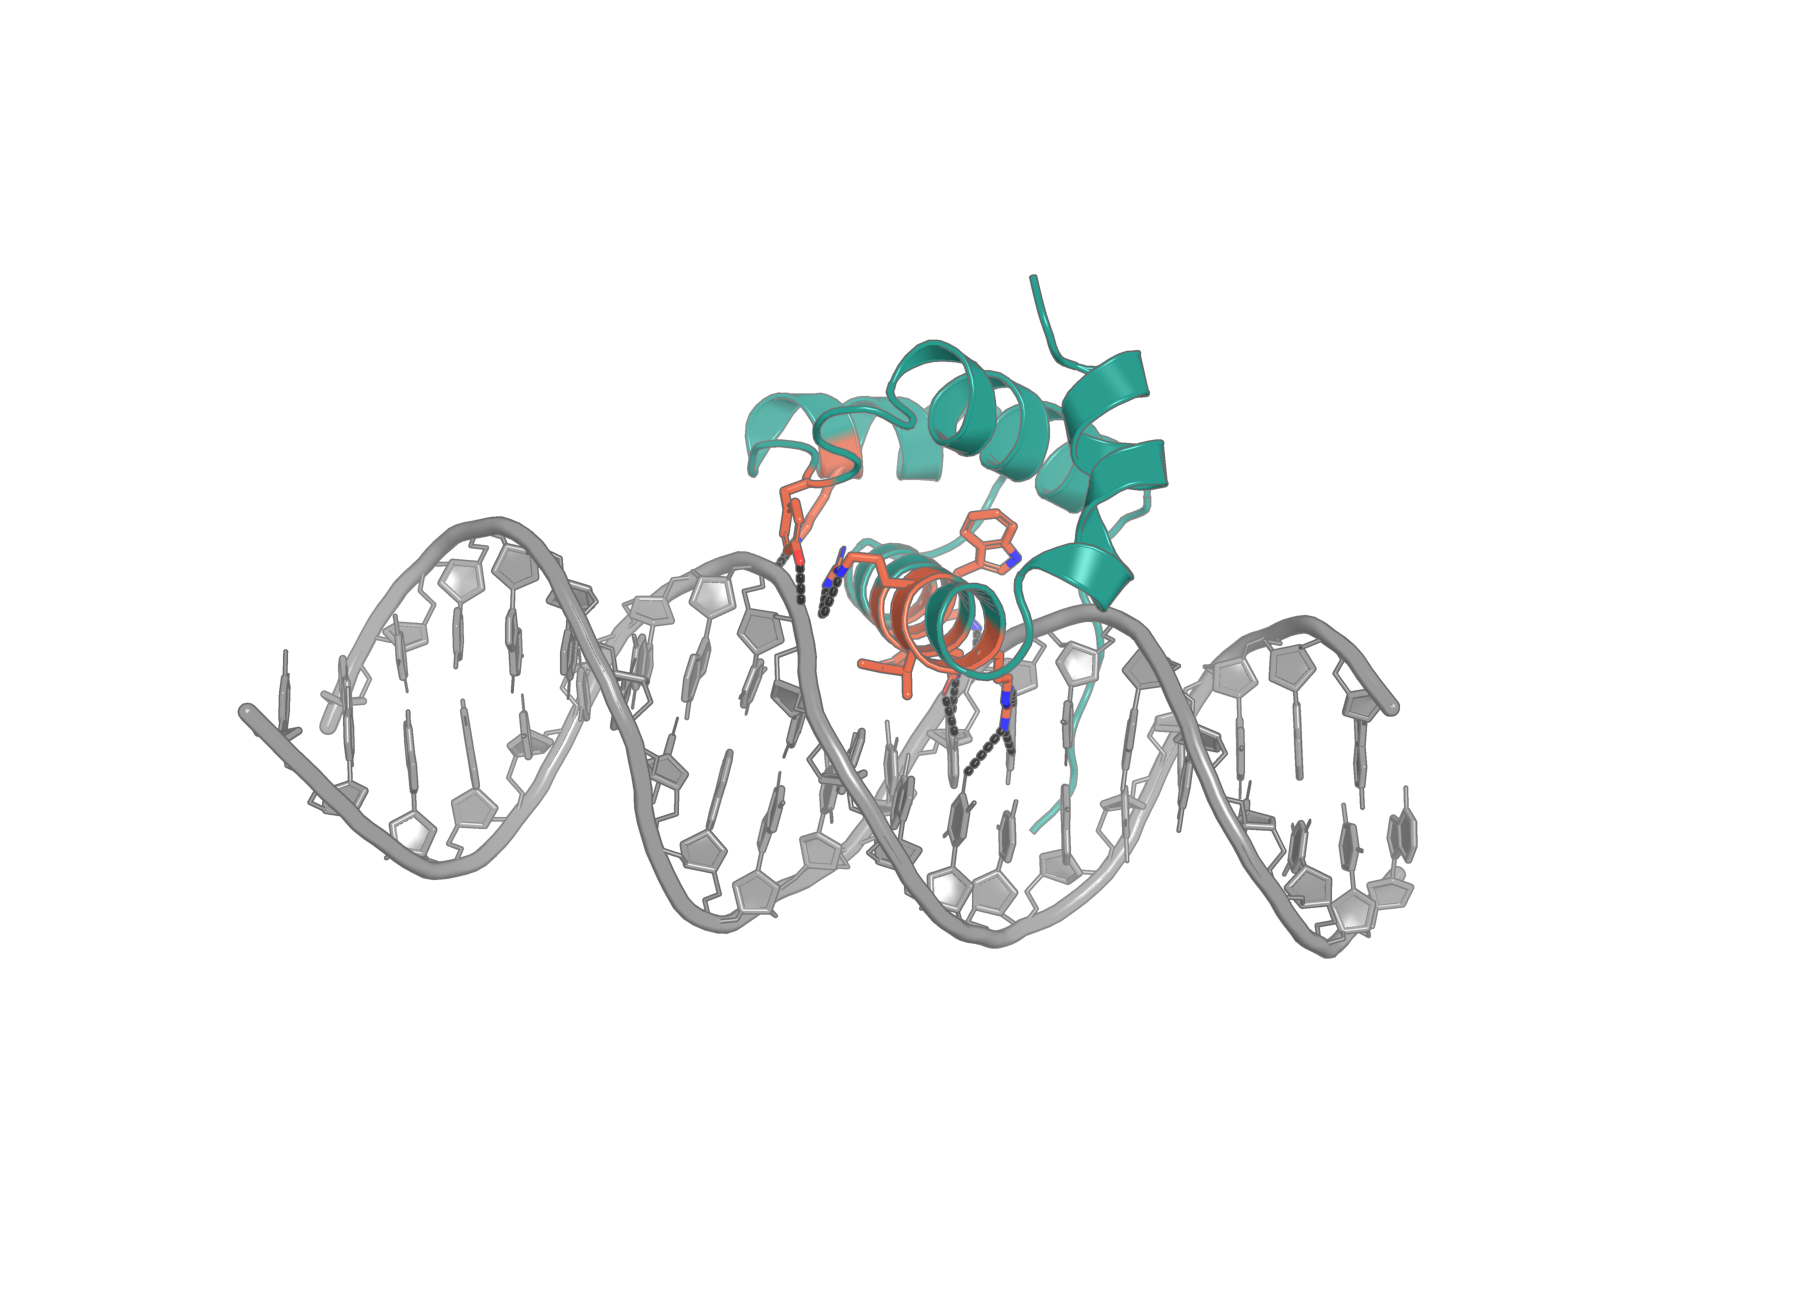
\includegraphics[width=0.6\linewidth]{recognition_pymol_1B72_PBX1.png}
\caption{\textbf{DNA-contact residues recognized by TFScope.} PBX1 homeodomain
(PDB 1B72): recognition-helix residues scored as DNA-contacting by the frozen-
backbone contact probe (AUROC $0.95$) shown as orange sticks with H-bonds to the
major-groove bases. \label{fig:recognition}}
\end{figure}

\begin{figure}[h]\centering

\includegraphics[width=0.85\linewidth]{figure2b_mutagenesis.png}
\caption{\textbf{In-silico mutagenesis / within-family signal.}
\TODO{finalize caption + add decomposition panel}. \label{fig:mutagenesis}}
\end{figure}

\begin{figure}[h]\centering

\includegraphics[width=0.7\linewidth]{figure4a_switch.png}
\caption{\textbf{Single-mutation motif switch.} MyoD1 L122R E-box switch,
$\Delta_{\mathrm{switch}}=+9.17$. \label{fig:switch}}
\end{figure}

\begin{figure}[h]\centering

\includegraphics[width=0.75\linewidth]{dbp_tfscope_heatmap.png}
\caption{\textbf{Designed DNA-binding proteins.} TFScope recovers intended CAC-
type preference (strongest DBP6, $r=0.65$). \label{fig:dbp}}
\end{figure}

% held-out recovery figure available: figure3a_heldout_clean.png (place where appropriate)

\clearpage
\bibliographystyle{unsrtnat}
\bibliography{../references/references}

\end{document}
